% \acrlong{AI}, which is abbreviated \acrshort{AI}
% or \gls{AI}

% Chapter 1
% 
\chapter{Introduction}
\label{chap:Chapter1}

This chapter will give the reader some context on what will be the main subject of this Master Thesis. The present work will be an attempt to tackle a problem presented by the literature: The scarcity of computational libraries that modulate \gls{CVNN} \parencite{bassey2021survey}, which will be diving deeply alongside with the main objectives on the up-coming sections.

\section{Contextualization}
\label{sec:chap1_context}
% contexto e problema descrição da estrutura

This Master Thesis explores a type of Neural Networks referred to as \gls{CVNN}. These are a computing systems, based on the way a biological brain operates. Despite being driven by data, the difference between CVNN and, for the sake of this work, \gls{RVNN}, is the fact that they incorporate complex numbers\footnote{Any number that belongs to the mathematical domain $\mathbb{C}$.} as their trainable or non-trainable parameters \parencite{clarke1990definition}. This can range from weights, biases or activation functions, but also the dynamics and operations involved inside the layers and even the training process itself, changes substantially.

This poses the question of why is it relevant to study these types of Networks? 

One of the first reasons, lies in the fact that, some data extracted by sensors, is inherently, complex-valued. Applications related to radar images of earth's surface \parencite{sunaga2019radar}, electromagnetic waves \parencite{mandic2009complex, hirose2012coherwave}, speech localization \parencite{tsuzuki2013approach} and MRI signals \parencite{virtue2017mribettercvnn}, data which is inherently represented in the complex domain, have already emerged with generally far greater results when compared to \gls{RVNN}. 

The second reason is because they offer more "expressiveness" \parencite{bassey2021survey, lee2022survey}, in other words, richer data representation that might encode more information related to a certain task. Matter of fact, \gls{CVNN} have also comparable or better performance when compared to \gls{RVNN}, in tasks where the input data is in the real domain, for instance in image classification \parencite{nafisah2018face}, segmentation \parencite{ceylan2013blood, saraswathi2014ensemble} and wind prediction \parencite{ccevik2018day}.

Finally, the third reason is a greater capacity for generalization \parencite{lee2022survey}. This fact becomes apparent in the results obtained by \parencite{zhang2021optical} where an extract can be visualized in Figure~\ref{fig:extract}.

\begin{figure}[htbp]
	\centering
	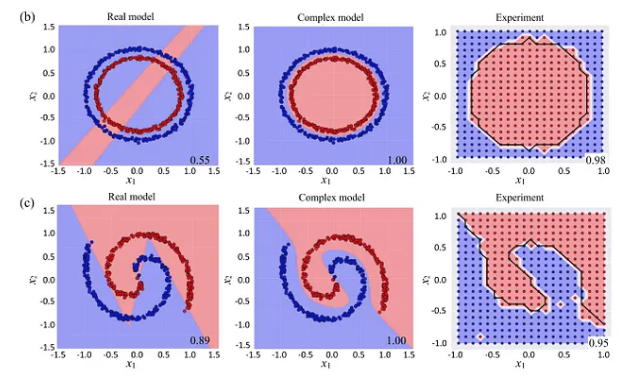
\includegraphics[width=1.\textwidth]{ch1/assets/extract.png}
	\caption{Portion of the results from the study \parencite{zhang2021optical}, that shows the generalization capabilities of a CVNN compared to a RVNN.}
	\label{fig:extract}
\end{figure}

\gls{RVNN} are more widely utilized since their implementation is considerably easier, there is a variety of tools to modulate them with little background knowledge, and less computationally expensive. Nevertheless, there is an untapped potential related to these \gls{CVNN} as it was alluded. \parencite{lee2022survey}. 

Furthermore, to give some fundamental context, complex numbers can be represented in the Euclidean form,
\begin{equation}
	z = x + iy,
\end{equation}
where $ \Real{z} = x $, $ \Imag{z} = y $ are respectively the real and imaginary component of $ z $, and $ i $ is the imaginary unit. Moreover, they can be represented in polar form,

\begin{equation}
	z = \rho e^{i \phi},
\end{equation}
where $ e $ is the Euler's constant, $ \rho = \sqrt{x^2 + y^2} $ is the absolute value and $ \phi = \arctan\left( \frac{y}{x} \right) $ is the phase of $ z $.  In this polar representation, a $ z $ number can represent an electromagnetic signal\footnote{This can be relevant for instance in fiber-optic or wireless communications.} with an amplitude of $ \rho $, and a phase $ \phi = \phi(t) = \omega t + \phi_0 $, being $ \phi_0 $ the initial phase. By having the time samples of a signal, one can perform tasks with a \gls{CVNN} with this signals as inputs or targets for instance. 

This improvement on performance, if taken out of context, might lead to a miss-conception that \gls{CVNN} are just \gls{RVNN} in two dimensions. The root of this misunderstanding stems from a viewing a complex number as two real numbers, which in fact, it is not. In \parencite{hirose2012coherwave}, it was proven otherwise that the multiplication of complex numbers, actually limits the degrees of freedom of the network, thus being something entirely different.

All these extra nuances may be able to represent, as it was stated by \textcite{hirose2012complex}, a "Super-Brain by Enrichment of the Information Representation". As it will become apparent, the engineering of complex activation functions and the various learning methods available for a CVNN are among the unique options not present in classical RVNNs. These innovations have the potential to significantly enhance performance in solving more challenging tasks.

\section{Problem Definition}
\label{sec:chap1_definition}

These networks were explored in a more theoretical level around 2012, and recently (2018 on-wards) some successful applications have been emerging. Nevertheless, this topic is underexplored, particularly in these CVNNs regarding the development of tools and libraries that allow one to explore such models \parencite{bassey2021survey}.

In that sense, there is a small number of tools and the already existent ones do not provide a solid foundation to model \gls{CVNN}s with close contact to its pipeline. Some were built on top of existing libraries meant for \gls{RVNN} modeling, while others discontinued with no further updates. Additionally, on this small list, there are publicly unavailable tools, which would be a drawback to the \gls{CS} community, given the already existence of extremely popular and reliable \gls{RVNN} open-source tools. Such tools will be reviewed, with more detail, in Chapter~\ref{sec:chap1_sota}.

\subsection{Objectives}

The objective of this Master Thesis is twofold:

\begin{itemize}
	\item Firstly, the main objective, is to build a library, which will be named Renplex, using the \href{https://www.rust-lang.org/}{Rust} programming language \parencite{rust2018}, which is capable of modeling these \gls{CVNN} with possibility to have as much control as possible over the ML pipeline. Such library will be public and released as an open-source project to tackle the problem described. Repository of this library can be found here \href{https://github.com/Pxdr0-A/renplex.git}{https://github.com/Pxdr0-A/renplex.git};
	\item Secondly, is to test some of the library's functionalities specifically in the comparison of performance between \gls{CVNN} and another popular library that models \gls{RVNN} \href{https://www.tensorflow.org/}{TensorFlow}. This is to ensure that it is working as intended and ready to be used for research and applications. \parencite{tensorflow2023}.  
\end{itemize}

The reason for choosing Rust as the programming language for this library, because it is a systems programming language that offers low-level memory management if needed with great performance and an emerging popularity \parencite{stackoverflow2023}. This makes it possible to produce a library capable of achieving some much needed runtime efficiency for network training, but specially, with notable scaling capabilities and security \parencite{rust2018}.

Additionally, Tensorflow is going to be the \gls{RVNN} modeling library for comparison due to being a very popular machine learning framework, but also a framework. On top of that, the author of this reasearch has more experience with it, thus minimizing execution errors. 

To meet these two objectives, there will be a set of tasks involved. On one hand, to allow for this customization, the library should ensure the ability to specify the precision of the calculations (32-bit or 64-bit float), provide a set of activation functions and layers to scaffold a personalized network. Ensuring these requirements, will allow to tackle the problem of the restrict \gls{CVNN} modeling.

On the other hand, to provide a concise comparison between \gls{CVNN} and \gls{RVNN}, the proposed pipeline will go as follows:

\begin{itemize}
    \item Only one optimization method will be explored for the \gls{CVNN}. This method the most analogous to the conventional back-propagation algorithm \parencite{rumelhart1986}: the fully back-propagation algorithm \parencite{barrachina2023theory}. For each dataset addressed in this Master Thesis, equivalent architectures between RVNN and CVNN will be trained and compared with each other's test performances;
    \item A special task regarding signal processing, where \gls{CVNN} typically out-perform will be considered to demonstrate that the developed models in the library are working as intended and in agreement with literature results.
\end{itemize}

This pipeline will ensure a fair comparison and demonstrate the usability of these \gls{CVNN}s, as a consequence, hopefully tackling the main problem of scarcity in viable \gls{CVNN} modeling tools in the open-source community for research purposes and real-world applications.
